\documentclass[a4paper,10pt]{report}

\usepackage{graphicx}
\usepackage{color}

\usepackage{caption}
\usepackage{subcaption}

\usepackage[portuguese]{babel}
\usepackage[utf8]{inputenc}
\usepackage[T1]{fontenc}

\usepackage{geometry}
\geometry{a4paper}
\usepackage[parfill]{parskip}

\usepackage{changepage}

\usepackage{amsmath}

\usepackage{fancyhdr}

\usepackage{nopageno}

\graphicspath{{./imagens/}}

\usepackage{url}

\usepackage{verbatim}
\usepackage{fancyvrb}

\usepackage[colorlinks=true,linkcolor=blue,citecolor=blue]{hyperref}

\usepackage{listings}
\renewcommand{\lstlistingname}{Código}
\usepackage{color}
\definecolor{grey}{rgb}{0.9,0.9,0.9}
\definecolor{greyD}{rgb}{0.5,0.5,0.5}

\lstnewenvironment{code}[1][]%
{
   \noindent
   \lstset{
	language=java,
	float=htpb,
	backgroundcolor=\color{grey},
	basicstyle=\scriptsize,
	numbers=left,
	numbersep=5pt,
	numberstyle=\tiny\color{greyD},
	breaklines=true,
	frame=single,
	#1}
}
{}

\begin{document}

\begin{titlepage}
\begin{center}

\begin{flushleft}

\includegraphics[height=3.00cm]{EENG.jpg}\\
\end{flushleft}

\vspace{2cm}

\Large{\textbf{LEI --- Licenciatura de Engenharia Informática}}\\
\vspace{1cm}
\Large{\textbf{UC8204P1 --- Programação Orientada a Objectos}}\\

\vspace{2.5cm}

\Huge{\textbf{FitnessUM}} \\

\vspace{2cm}

\Large{\textbf{Grupo XXXX}}\\
\vspace{0.5cm}
\normalsize{\textbf{Rui Camposinhos - a72625, Rui Oliveira - a67661, André Santos - a61778}}\\
\vspace{0.5cm}
\begin{figure}[h]
\centering
\begin{subfigure}{.2\textwidth}
  \centering
  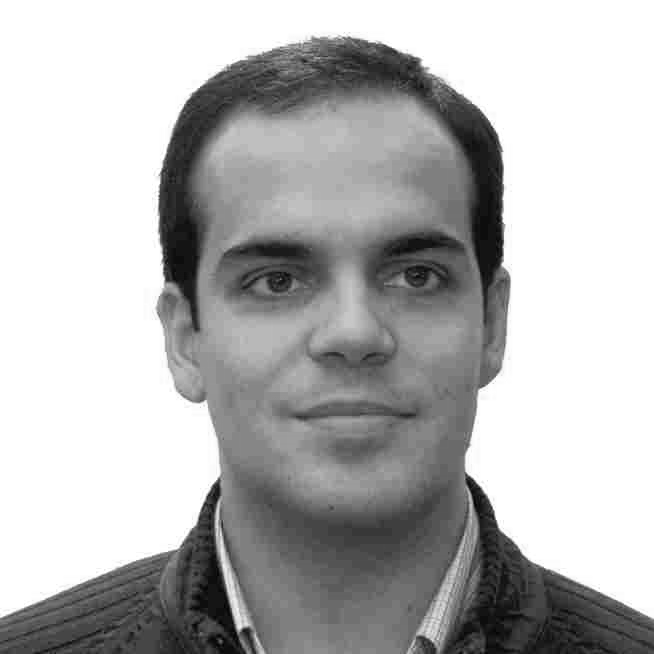
\includegraphics[width=\textwidth]{Camposinhos.jpg}
\end{subfigure}
\begin{subfigure}{.2\textwidth}
  \centering
  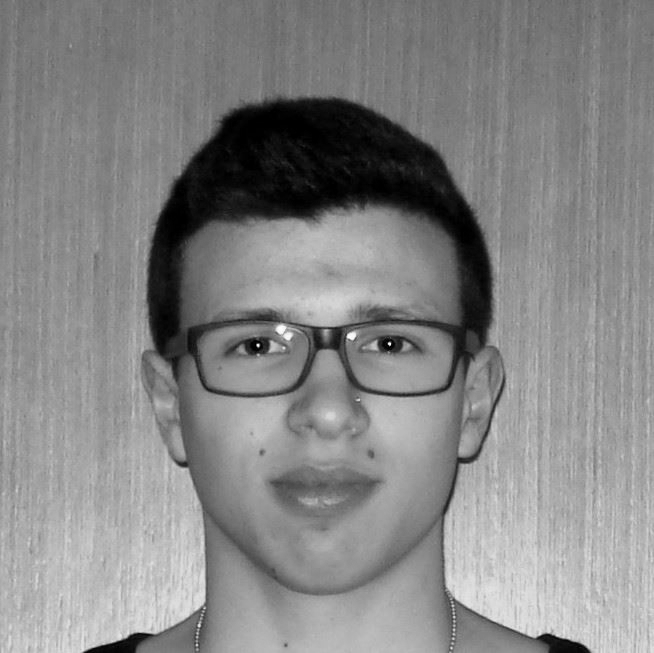
\includegraphics[width=\textwidth]{Oliveira.jpg}
\end{subfigure}
\begin{subfigure}{.2\textwidth}
  \centering
  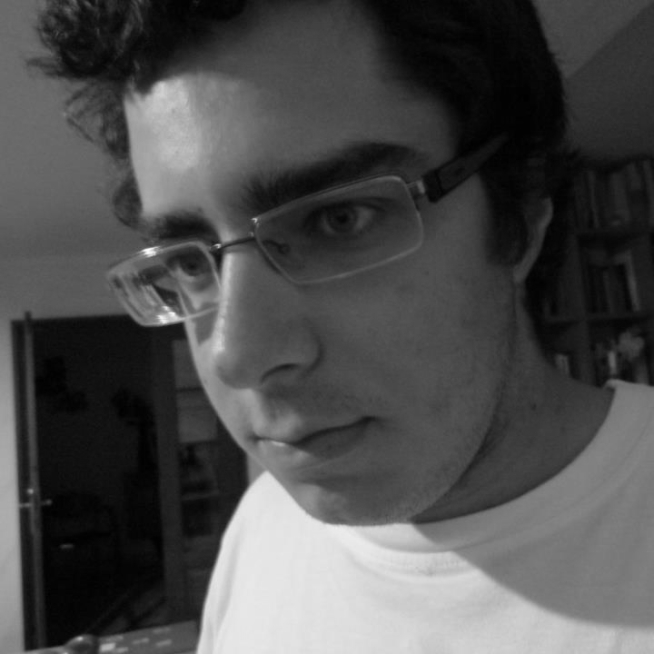
\includegraphics[width=\textwidth]{Santos.jpg}
\end{subfigure}
\end{figure}

\vspace{2cm}
Braga, 1 de junho de 2014

\end{center}

\end{titlepage}
%----------------------------------------------------------------------
\newpage
\phantom{placeholder} % doesn't appear on page
\thispagestyle{empty} % if want no header/footer
%----------------------------------------------------------------------
\tableofcontents
\phantom{placeholder} % doesn't appear on page
\thispagestyle{empty} % if want no header/footer
%----------------------------------------------------------------------
\newpage
\phantom{placeholder} % doesn't appear on page
\thispagestyle{empty} % if want no header/footer
%----------------------------------------------------------------------
\pagestyle{fancy}
\setlength{\headheight}{15.2pt}
\fancyhf{} % apagar as configurações actuais
\fancyfoot[LE,RO]{\thepage}
\fancyhead[LE,RO]{POO --- FitnessUM --- Grupo 14}
\setcounter{page}{0}
%----------------------------------------------------------------------

\chapter{Introdução}
\label{cap:intro}
O presente projecto enquadra-se na unidade curricular de Programação Orientada a Objectos do curso de Licenciatura em Engenharia 
Informática da Universidade do Minho.
O projecto pretende implementar uma aplicação, designada \emph{FitnessUM}, para registar e simular actividades desportivas.
A aplicação foi desenvolvida na linguagem \emph{java} e pretende simular um ambiente de rede social.

\section{Objectivos}
\label{sec:obj}
O presente projeto tem como objectivo principal consolidar e colocar em práctica os conceitos fundamentais transmitidos durante a UC de 
Programação Orientada a Objectos.

De acordo com o enunciado \cite{enunciado}, os principais objectivos definidos para a aplicação \emph{FitnessUM} são os seguintes:

\textbf{Requisitos básicos}
\begin{itemize}
\item Aceder à aplicação utilizando as credenciais (email e password);
\item Visualizar a informação das actividades, do próprio e dos amigos, com possibilidade de aceder aos seus detalhes; 
\item Registar a informação de uma actividade;
\item Consultar, por ordem cronológica, e remover actividades;  
\item Aceder às estatísticas de distância, tempo e calorias gastas;
\end{itemize}

\textbf{Requisitos de valorização}
\begin{itemize}
\item Definir tipos de recordes e registar os recordes pessoais de cada utilizador;
\item Definir eventos e proceder à sua simulação a partir dos administratores da aplicação.
\end{itemize}

\section{Organização do Relatório}
\label{sec:org}
O presente relatório serve de suporte à aplicação desenvolvida, apresentando uma descrição geral dos aspectos mais importantes.
Com excepção do presente capítulo introdutório, o relatório é composto por dois capítulos iniciais e nucleares  - Arquitectura e 
Estruturas de Dados - e por quatro capítulos complementares relacionados com funcionalidades particulares da aplicação - Consumo de Calorias, 
Forma dos Utilizadores, Estatísticas e Simulação de Eventos. No final são tecidas algumas conclusões, bem como apresentadas algumas imagens da
aplicação em anexo.

\chapter{Arquitectura e Descrição da Aplicação}
\label{cap:arq}

A aplicação foi desenvolvida utilizando simultaneamente os IDEs \emph{Eclipse} e \emph{BlueJ}.

Foi utilizada uma arquitectura do tipo \emph{Model–View–Controller} (MVC) - ver figura \ref{fig:mvc} -, 
permitindo uma interface gráfica com o utilizador.

De forma a manter uma estrutura de pastas partilhada entre os autores e um controlo de versões eficaz, 
foi utilizada a ferramenta open source \emph{GIT} (\url{http://git-scm.com/}), 
com repositório privado no bitbucket (\url{https://bitbucket.org/ruiOliveiras94/fitnessum-poo}).

\begin{figure}
\centering
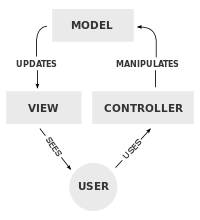
\includegraphics[width=4cm]{MVC-Process.png}
\caption{Diagrama com a relação típica dos componentes do MVC (ref.:\url{http://en.wikipedia.org/wiki/Model-view-controller}).}
\label{fig:mvc}
\end{figure}

\section{Packages}
\label{sec:packages}
A figura \ref{fig:src} apresenta os packages principais da aplicação, em correspondência com a arquitectura MVC descrita.

Na figura \ref{fig:model} descreve o package \emph{model}, com os seus sub-packages principais - activity, user e events -, 
bem como \emph{Dataset} para gestão dos dados e a classe para definição dos recordes (ver \ref{sec:record}).
A classe \emph{Dataset} é o conjunto de toda a informação referente à aplicação criada, 
contendo um conjunto de utilizadores e outro de eventos. 
Esta informação é acedida através da classe \emph{Manager}, descrita na secção \ref{sec:manager}.

O package \emph{model}, descrito na figura \ref{fig:view}, gere toda a interface gráfica com o utilizador.

O package \emph{controller} encontra-se descrito na figura \ref{fig:controller}, possuindo todas as classes de controlo da aplicação, 
bem como a classe principal (Main) com o executável da aplicação.

O package \emph{core}, descrito na figura \ref{fig:core}, foi criado para alojar algumas funcionalidades mais especificas da aplicação.
A sua separação dos packages principais deveu-se unicamente a uma opção de organização e gestão do código, 
assim como para facilitar o desenvolvimento em paralelo por parte dos diferentes autores.
Neste package inclui-se o código desenvolvido para o cálculo de calorias, cálculo da forma, cálculo de estatísticas e métodos de simulação.
Todos os métodos foram implementados como \verb!static!.

\begin{figure}
\centering
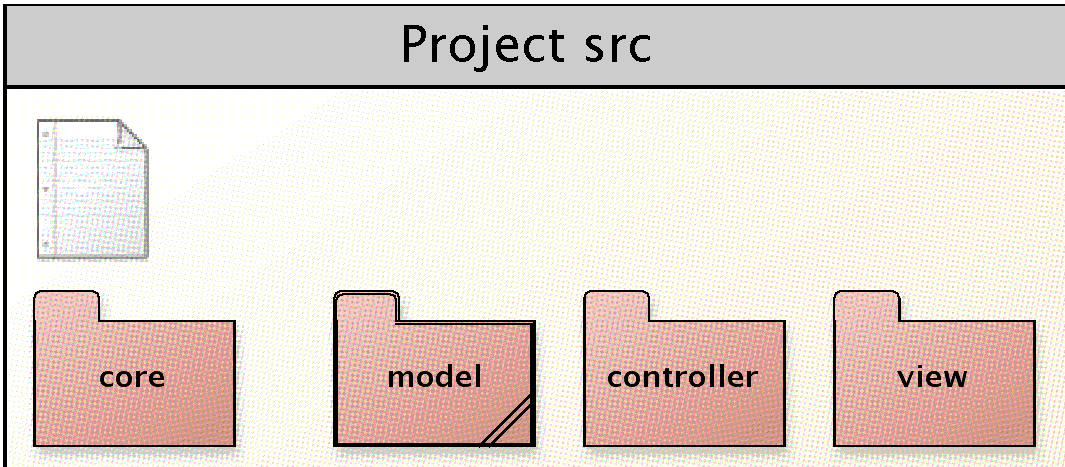
\includegraphics[width=7cm]{src.png}
\caption{Pasta \emph{source} com os vários \emph{packages} desenvolvidos.}
\label{fig:src}
\end{figure}

\begin{figure}
\centering
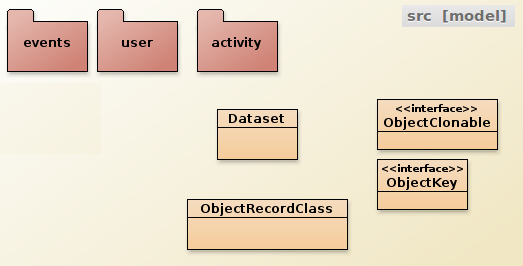
\includegraphics[width=7cm]{model.png}
\caption{\emph{Package model} (src/model).}
\label{fig:model}
\end{figure}

\begin{figure}
\centering
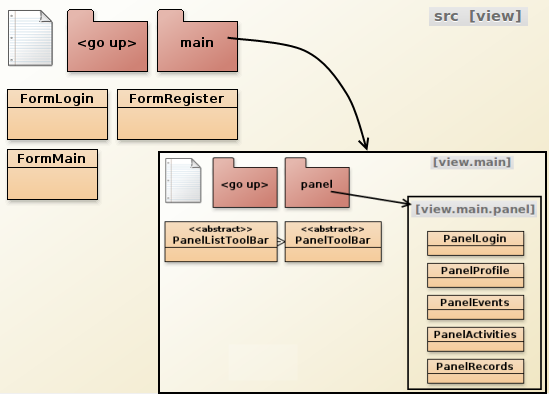
\includegraphics[width=7cm]{view.png}
\caption{\emph{Package view} (src/view).}
\label{fig:view}
\end{figure}

\begin{figure}
\centering
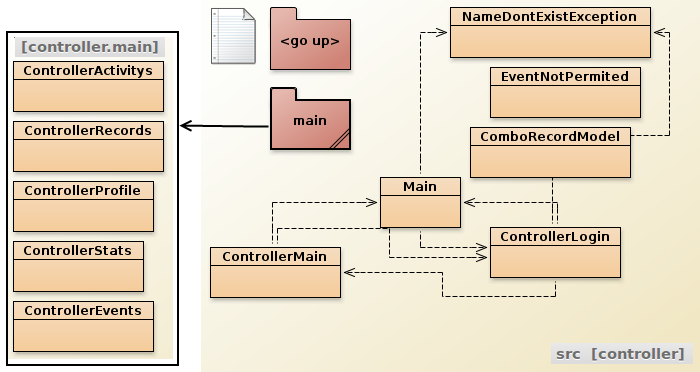
\includegraphics[width=7cm]{controller.png}
\caption{\emph{Package controller} (src/controller).}
\label{fig:controller}
\end{figure}

\begin{figure}
\centering
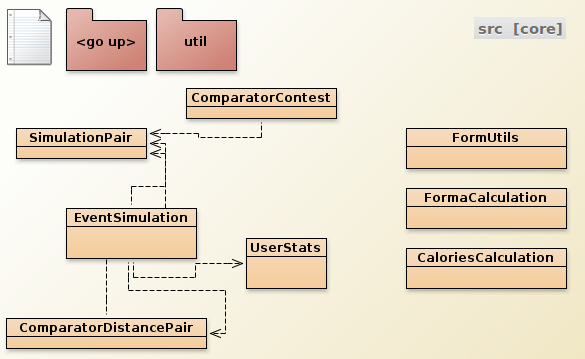
\includegraphics[width=7cm]{core.png}
\caption{\emph{Package core} (src/core).}
\label{fig:core}
\end{figure}

\section{Encapsulamento: Manager}
\label{sec:manager}
A figura \ref{fig:manager} apresenta o diagrama de classes relativo ao \emph{Manager}.

A classe Manager foi criada para facilitar o encapsulamento de tipos \verb!Map! ou \verb!Set!, e realiza as operações básicas de gestão 
(na adição faz um clone, na pesquisa retornar um clone).

Quando se instancia a classe \emph{Manager}, passa-se a estrutura que pretendemos encapsular, a partir daí esta estrutura nunca mais 
pode ser acedida. Assim, caso seja necessária aceder a algum método especifico da estrutura, antes de esta ser instanciada deverá ser guardada.

Desta forma torna-se suficiente retornar o \emph{Manager} para que o exterior consiga aceder de forma encapsulada à informação.

Para se poder utilizar um \emph{Manager} de \verb!Map! os objetos devem implementar a interface \emph{ObjectKey}. 
O valor retornado por essa função será a chave do objecto no \verb!Map!.

\begin{figure}
\centering
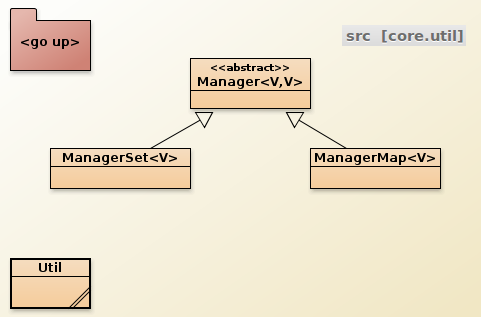
\includegraphics[width=7cm]{coreUtil.png}
\caption{\emph{Package} util (src/core/util) com o \emph{Manager} de colecções.}
\label{fig:manager}
\end{figure}

\section{Diagramas de Classes}
\label{sec:classes}
\subsection{Actividades}
\label{subsec:actividadesDiagrama}
Na figura \ref{fig:activityTable} apresentam-se todas as actividades físicas implementadas na aplicação, 
bem como as constantes especificas de cada clasee \verb!MET! e \verb!Intensidade!, que serão descritas adiante.
As actividades foram todas classificadas em um de cinco tipos: Distance, Altimetry, Skill, Ludic e Contest.
As estruturas de dados de cada classe encontram-se descritas no capítulo \ref{cap:estruturas}.

As classes de actividades físicas para além de funcionarem como um modelo de classificação, 
obedecem a uma hierarquia, onde são herdados atributos e ``obrigações'' das classes hierárquicamente superiores.
A figura \ref{fig:activityDiagram} apresenta o diagrama de classes de actividades, obtido através do \emph{BlueJ}.
A hierarquia de classes definida implica a herança de alguns métodos abstractos fundamentais para a aplicação.
São exemplo disso os método \verb!getIntensidade()! e o \verb!getMET()!.
O primeiro devolve o número de minutos diários recomendados para a actividade, para que o utilizador atinga uma forma ideal. 
O segundo, serve de base ao cálculo das calorias dessa actividade, devolvendo uma constante específica de cada actividade (ver secção \ref{sec:caloriasMet}).

\begin{figure}
\centering
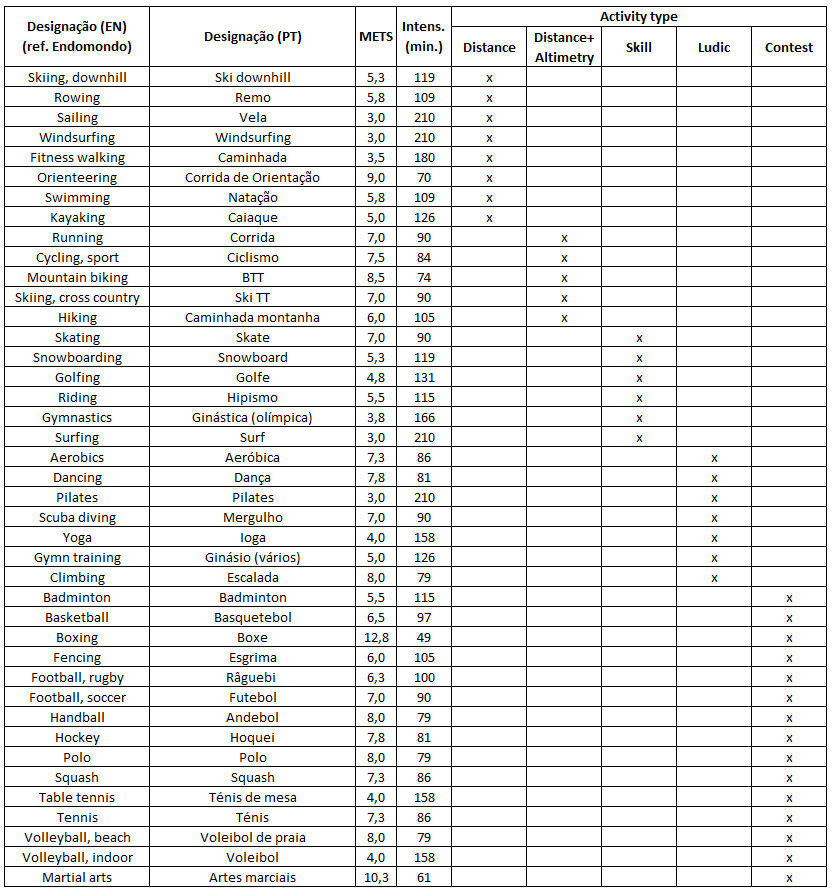
\includegraphics[width=\textwidth]{activitiesTable.png}
\caption{Lista de actividades implementadas na aplicação.}
\label{fig:activityTable}
\end{figure}

\begin{figure}
\centering
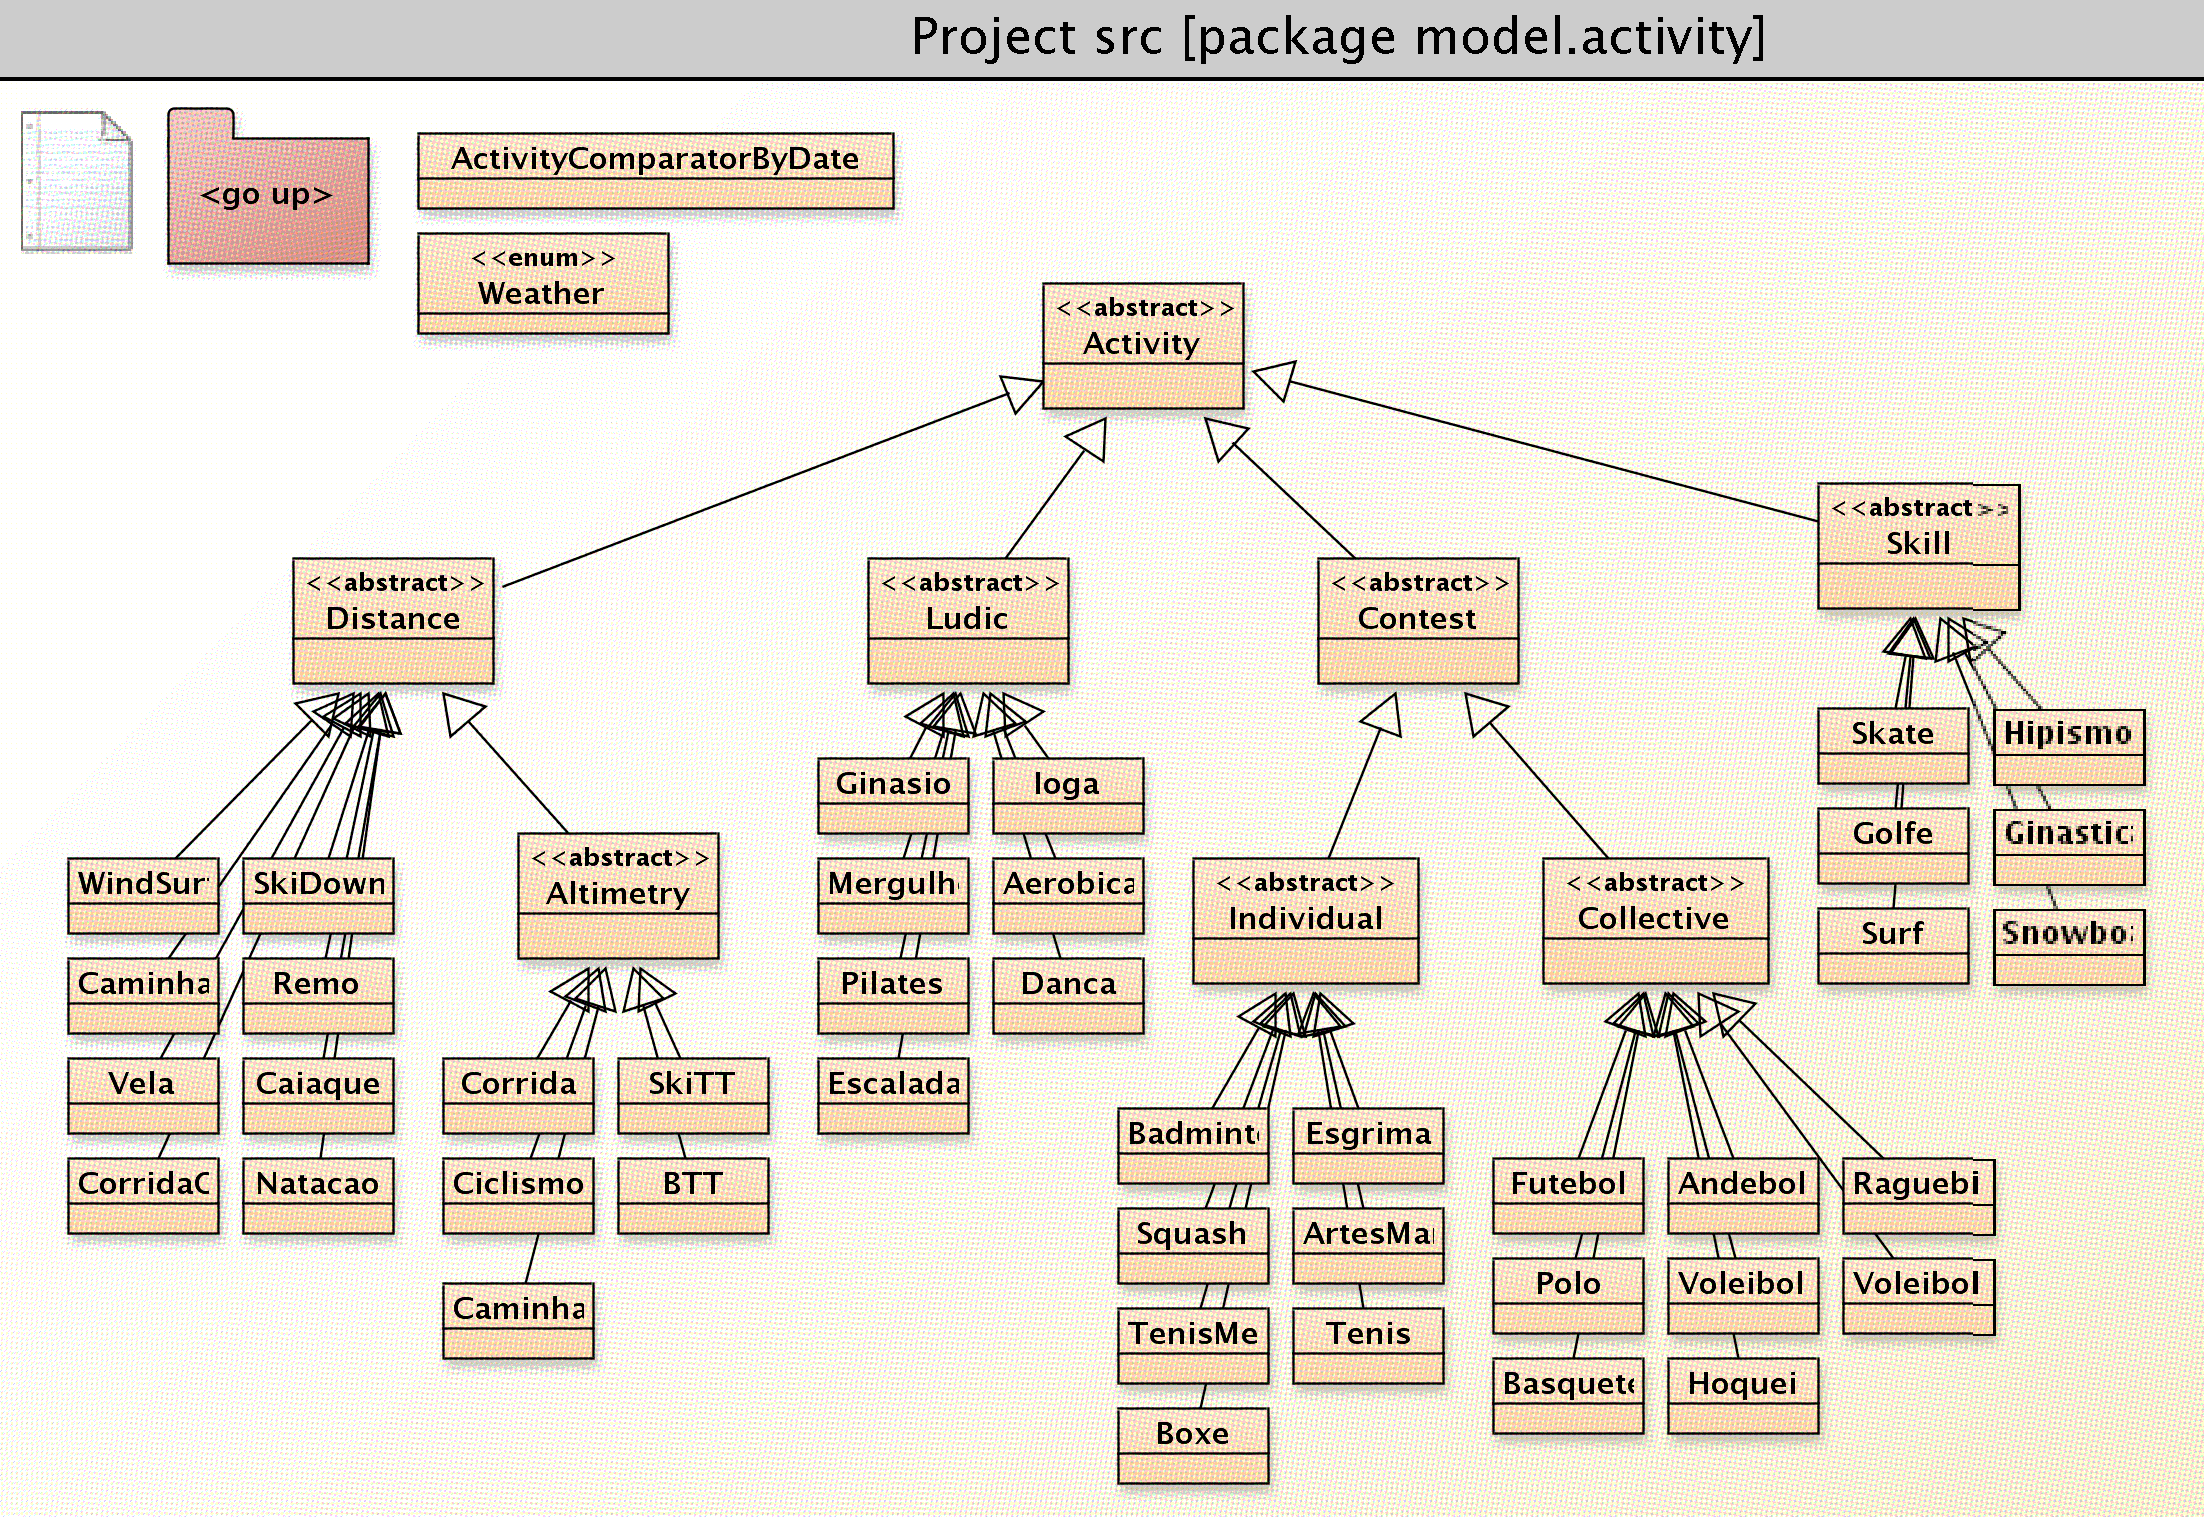
\includegraphics[width=\textwidth]{diagramaActivities.png}
\caption{Diagrama com dependências da super classe \emph{Activity} (src/model/activity).}
\label{fig:activityDiagram}
\end{figure}

\subsection{Eventos}
\label{subsec:eventosDiagrama}
Para além das actividades, também os eventos obedecem a uma hierarquia.
As estruturas de dados de cada classe de evento encontram-se descritas no capítulo \ref{cap:estruturas}.
De forma semelhante às actividades, embora mais simplificada, definiram dois tipos de eventos: Distance e Contest.
A figura \ref{fig:eventDiagram} descreve essas dependências.

\begin{figure}
\centering
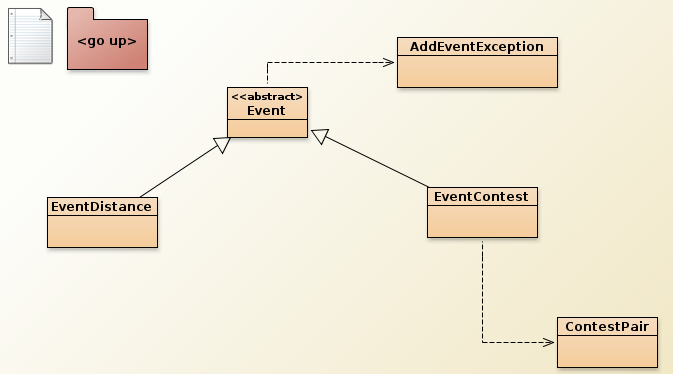
\includegraphics[width=10cm]{events.png}
\caption{Diagrama com dependências da super classe \emph{Event} (src/model/events).}
\label{fig:eventDiagram}
\end{figure}

\section{Funcionalidades da Aplicação}
\label{sec:funcionalidades}
A aplicação desenvolvida apresenta um conjunto considerável de funcionalidades, sendo de destacar as seguintes:

\begin{itemize}
 \item Interface gráfica com o utilizador;
 \item Registo de novos utilizadores com credenciais;
 \item Possibilidade de registar actividade em 41 modalidades;
 \item Amizades entre utilizadores (dependendo da aceitação de convites);
 \item Apresentação de índice evolutivo de forma em função das actividades registadas;
 \item Cálculo das calorias dispendidas em função do género e características físicas de cada índividuo, 
	  por intermédio da frequência cardíaca ou tipo de actividade;
 \item Apresentação de estatísticas de actividades em termos de duração, calorias e distância percorrida;
 \item Criação e simulação de eventos de distância ou do tipo torneio;
 \item Possibilidade de extensibilidade para novas actividades e eventos.
\end{itemize}

\chapter{Estruturas de Dados Principais}
\label{cap:estruturas}
\section{User class}
\label{sec:user}
As variáveis de instância da classe \verb!User! são apresentadas no excerto de código \ref{code:user}.
Na figura \ref{fig:user} apresenta-se o package respetivo.
Para as permissões foi usada uma enumeração correspondente aos diferentes tipos de utilizador. 
Estas permissões são usadas para controlar as funcionalidades a que o utilizador tem acesso na aplicação.
Para os recordes foi usado um \verb!Map! de uma classe correspondente a uma modalidade para o conjunto de recordes dessa modalidade. 
Um recorde é constituído pelo seu tipo, dado por um inteiro e por uma ``Actividade modelo'', que representa o recorde.
Para os amigos e lista de amigos foi utilizado o \verb!Manager!, que é instanciado numa \verb!HashSet! de \verb!String!.
Para o conjunto de actividades realizadas, foi também utilizado o Manager instanciado numa árvore (TreeSet), ordenado por meio 
de um \verb!Comparator!, que compara as actividades por ordem crescente da sua data de realização.

\begin{figure}
\centering
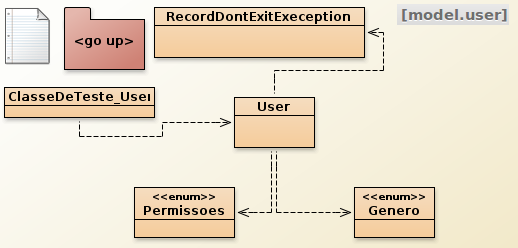
\includegraphics[width=7cm]{user.png}
\caption{\emph{Package user}  (src/model/user).}
\label{fig:user}
\end{figure}

\begin{code}[caption=Variáveis de instância da classe User (src/model/user)., label=code:user]
private String email;
private String nome;
private String password;
private Genero genero;
private int altura; /*cm*/
private int peso; /*kg*/
private GregorianCalendar dataNascimento;
private Activity desportoFavorito;
private Permissoes permissoes;
private Map<Class<?>, HashMap<Integer, Activity>>  recordes; /*ver documentacao*/
private int fcr; /*frequencia cardiaca em repouso - para calculo das calorias*/
private Manager<String> amigos; /*emails amigos:HashSet com chaves para rede social*/
private Manager<String> convitesAmigos; /*emails de amigos: convites - HashSet*/
private Manager<Activity> actividadesUser; /*Actividades do User:TreeSet -Comp.ByDate*/
\end{code}

\section{Activity class}
\label{sec:activity}
Na superclasse abstracta \verb!Activity! foram incorporadas todas as variáveis de instância e métodos gerais das actividades, 
designadamente a data, duração, meteorologia e frequência cardíaca média durante a actividade, caso seja fornecida pelo utilizador.
Para as condições meteorológicas foi usada uma enumeração para cobrir as situações mais frequentes em termos de clima.
Num nível hierárquico abaixo da superclasse surgem as subclasses \verb!Distance!, \verb!Altimetry!, \verb!Contest!, \verb!Skill! e \verb!Ludic!.

A subclasse \verb!Distance! especializa a superclasse com duas variáveis de instância relativas a actividades que envolvam distâncias, a saber a 
distância percorrida e a velocidade atingida no percurso.
A subclasse \verb!Altimetry! descende da subclasse \verb!Distance!, acrescentando atributos às actividades que além de terem distância têm associada altura, 
nomeadamente a distância que foi subida e descida, bem como as altitudes máxima e mínima atingidas.
A subclasse \verb!Contest! descende da superclasse e representa as actividades em que esteja envolvido algum tipo de disputa/jogo (de equipa ou individual).
As suas variáveis de instância representam os pontos obtidos pela equipa adversária e pela própria equipa.
A subclasse \verb!Skill! representa as actividades em que a performance é avaliada em termos de uma pontuação, através de uma exibição individual.
As variáveis de especialização são a pontuação final obtida e o máximo de pontuação obtida para um determinado movimento.
A subclasse \verb!Ludic! representa actividades mais simples e com um carácter mais lúdico. Esta classe não apresenta nenhum especialização relativamente à 
superclasse. Para além dos métodos abstractos impostos pela superclasse, são também definidos nesta classe os tipos de recordes específicos.
Todas as variáveis da superclasse e subclasses referidas são apresentadas no excerto de código \ref{code:activity}.

\begin{code}[caption=Variáveis de instância da superclasse Activity e subclasses respectivas (src/model/activity)., label=code:activity]
/***Super Classe***/
private GregorianCalendar mDate;
private long mDuration; /*activity duration [ms]*/
private Weather mWeather;
private int mHearthRate;/*heart rate [1/min] - for calorie burn calculation*/

/**Especializacoes Classe Distance**/
private int mDistance;
private int mMaxSpeed;

/**Especializacoes Classe Contest**/
private int mPointRival;
private int mPointTeam;
private Contest.Result mResult;

/**Especializacoes Classe Skill**/
private int mPoints;
private int mMaxTrick;
\end{code}

\section{Mecanismo para Recordes}
\label{sec:record}
Os recordes das Actividades foram organizados da seguinte forma: todas as actividades implementam \verb!ObjectRecord!, e em cada actividade 
tem uma enumeração de \verb!Records! e outra com os \verb!EnumAttr!.
Os \verb!Records! e os \verb!EnumAttr! devem ser acedidos através dos métodos da interface \verb!ObjectRecord!.

Quando uma actividade extende a outra (exemplo: \verb!Altimetry! extende a \verb!Distance!), 
os métodos de acesso aos \verb!Records! do objecto funcionam da seguinte forma:
\begin{itemize}
 \item Se o recorde estiver definido naquela Actividade encontrou e pára;
 \item Caso contrario pesquisa no nível seguinte
\end{itemize}

\subsection{Record interface}
\label{subsec:record}
A interface \verb!Record! representa um tipo de recorde e é caracterizado por:
\begin{itemize}
 \item Um Nome e um ID. 
 \item Um atributo principal, que é atributo que irá ser medido.
 \item Um atributo fixo (opcional), que funciona como constante para criar recordes semelhantes, mas com um valor diferente 
	(exemplo: \"recorde de tempo em X metros\", X pode é visto como um atributo fixo).
\end{itemize}

Esta interface também oferece a funcionalidade de verificar, quando necessário, se um valor de um atributo é semelhante ao valor do atributo fixo.

\subsection{EnumAttr interface}
\label{subsec:enumAttr}
A interface \verb!EnumAttr! representa um atributo, é caracterizado por um Nome e um ID. 
Esta interface permite aceder aos atributos de forma genérica.

\subsection{ObjectRecord interface}
\label{subsec:objectRecord}
A interface \verb!ObjectRecord! representa uma entidade constituída por vários recordes. 
Assim, um objecto que implemente \verb!ObjectRecord! terá as seguintes funcionalidades:

\begin{itemize}
 \item Porta de acesso para os recordes através do seu ID.
 \item Porta de acesso para os atributos através do seu ID.
 \item Ser comparado com outro \verb!ObjectRecord!, para um determinado \verb!Record!, e saber qual é o melhor.
 \item Representar este \verb!ObjectRecord! para um determinado \verb!Record! sobe a forma de String.
\end{itemize}

\section{Event class}
\label{sec:event}
As variáveis de instância da superclasse \verb!Event! são apresentadas no excerto de código \ref{code:event}.
Um evento pode ser caracterizado pelo seu nome, actividade associada, tipo de recorde associado, 
data de início e término, um valor correspondente a um pré-requisito necessário que um utilizador possa aderir ao evento, 
o número máximo de utilizadores que o evento suporta e o número de utilizadores actualmente inscritos.
Os eventos são também classificados em dois tipos: de distância, ou do tipo torneio (jogos).
As subclasses que traduzem essa classificação são a subclasse \verb!EventDistance! e \verb!EventContest!.

\begin{code}[caption=Variáveis de instância da superclasse Event e subclasses respectivas (src/model/event)., label=code:event]
/***Super Classe***/
private String mName;
private Activity mActivity;/*ATENTION: event weather inside activity*/
private int mRecordType;
private GregorianCalendar mEventDate;
private GregorianCalendar mEndDate;/*deadline for joining*/
private long mPreRequisite;
private int mMaxNumUsers;
private ManagerSet<String> mUsers; /*HashSet ok User keys(emails)*/

/**Especializacoes Classe EventDistance**/
private int mEventDistance;/*An event is about a Activity with its record type, like: Run 10000m*/

/**Especializacoes Classe Contest**/
private int mNum;/*Legs Between Users (1 Leg = 2 games)*/
private int mPointsVic;
private int mPointsDraw;
private int mPointsLoss;
\end{code}

\chapter{Cálculo do Consumo de Calorias por Actividade}
\label{cap:calorias}
O procedimento de cálculo utilizado para estimar a quantidade de calorias dispendidas por actividade seguiu uma filosofia semelhante à utilizada 
na rede social \emph{Endomondo} (\url{www.endomondo.com}). 
Na figura \ref{fig:caloriasProcedimento} apresenta-se um diagrama explicativo do mesmo, onde se evidenciam duas vias: uma baseada na frequência 
cardíaca e outra no tipo de actividade.

Os dados básicos necessários para o cálculo das calorias dispendidas estão relacionados com o individuo e são:
\begin{itemize}
 \item Género;
 \item Características físicas --- peso, altura;
 \item Idade;
 \item Frequência cardíaca em repouso (no caso da via de cálculo baseada na frequência cardíaca).
\end{itemize}

Os dados complementares são:
\begin{itemize}
 \item Duração da actividade;
 \item O tipo de actividade (no caso da via de cálculo baseada no tipo de actividade);
 \item Frequência cardíaca média durante a actividade (no caso da via de cálculo baseada na frequência cardíaca).
\end{itemize}

\begin{figure}
\centering
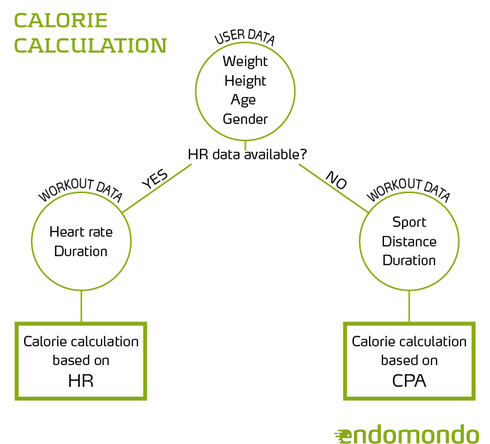
\includegraphics[width=7cm]{endomondoCalories.jpg}
\caption{Diagrama com o procedimento de cálculo adoptado para a estimativa do consumo de calorias por actividade (ref. \cite{endomondo}).}
\label{fig:caloriasProcedimento}
\end{figure}

\section{Cálculo Baseado na Frequência Cardíaca}
\label{sec:caloriasFcardio}
As formulações expostas na presente secção tiveram por base a aplicação web ``Heart Rate Based Calorie Burn Calculator'', 
da página \url{http://www.shapesense.com/fitness-exercise/calculators/}. Por uma questão de completitude apresentam-se todas as referências originais.
No cálculo pela via da frequência cardíaca um dos parâmetros fundamentais é o $VO2_{max}$, que é a capacidade máxima do corpo de um 
indivíduo em transportar e fazer uso de oxigênio durante um exercício físico incremental.
Este parâmetro pode ser estimado de acordo com \cite{VO2max}, com base na frequência cardíaca máxima ($MHR$) e em 
repouso ($RHR$) --- equação \ref{eq:VO2max}.
A frequência cardíaca máxima pode ser estimada com base na idade de acordo com \cite{MHR} --- equação \ref{eq:MHR}.
As calorias brutas dispendidas ($GCB$) foram estimadas de acordo com \cite{GCB} --- equação \ref{eq:GCB}.
Por fim, para se determinar o número de calorias efectivas ($NCB$) calculou-se a taxa metabólica basal ($BMR$) e a taxa de actividade ($RMRCB$)
A estimativa das calorias efectivas foi realizada de acordo com \cite{NCB} --- equações \ref{eq:NCB}, \ref{eq:RMRCB} e \ref{eq:BMR}.

\begin{equation} \label{eq:MHR} 
MHR = 208 - 0.7 \times Idade \text{\hspace*{0.3cm}[1/min]}
\end{equation}

\begin{equation} \label{eq:VO2max} 
VO2_{max} = 15.3 \times \frac{MHR}{RMR} \text{\hspace*{0.3cm}[ml/(kg.min)]}
\end{equation}

\begin{eqnarray} \label{eq:GCB}
\text{Homens:}&&\\ 
GCB &=& \frac{-55.0969 + 0.6309 \times HR + 0.1988 \times W + 0.2017 \times A}{4.184} \times 60 \times T \text{\hspace*{0.3cm}[kcal]}\nonumber\\
\text{Mulheres:}&&\nonumber\\ 
GCB &=& \frac{-20.4022 + 0.4472 \times HR + 0.1263 \times W + 0.074 \times A}{4.184} \times 60 \times T \text{\hspace*{0.3cm}[kcal]}\nonumber\\
\text{onde:}&& \nonumber\\
HR &=& \text{frequência cardíaca [1/min]}\nonumber\\ 
W &=& \text{Peso [kg]}\nonumber\\
A &=& \text{Idade [anos]}\nonumber\\
T &=& \text{Duração exercício [h]}\nonumber
\end{eqnarray}

\begin{equation} \label{eq:NCB} 
NCB = GCB - RMRCB \text{\hspace*{0.3cm}[kcal]}
\end{equation}

\begin{equation} \label{eq:RMRCB} 
RMRCB = \frac{BMR \times 1.1}{24} \times T \text{\hspace*{0.3cm}[kcal]}
\end{equation}

\begin{eqnarray} \label{eq:BMR}
\text{Homens:}&&\\
BMR &=& (13.75 \times W) + (5 \times H) - (6.76 \times A) + 66 \text{\hspace*{0.3cm}[kcal/24h]}\nonumber\\
\text{Mulheres:}&&\nonumber\\ 
BMR &=& (9.56 \times W) + (1.85 \times H) - 4.68 \times A) + 655 \text{\hspace*{0.3cm}[kcal/24h]}\nonumber\\
\text{onde:}&& \nonumber\\
H &=& \text{altura [cm]}\nonumber\\ 
&&\text{restantes referências na eq. \ref{eq:GCB}}\nonumber
\end{eqnarray}

\section{Cálculo Baseado no Tipo de Actividade}
\label{sec:caloriasMet}
Na ausência de dados relativos à frequência cardíaca do individuo, o cálculo do número de calorias dispendidas ($CB$) é efectuado com base 
no índice MET (``The Metabolic Equivalent of Task''). Este índice é uma medida fisiológica do custo energético de um dado exercício físico.
Com base nesta abordagem mais simplificada, as calorias dispendidas podem ser calculadas de acordo com a equação \ref{eq:CBmet}.

\begin{equation} \label{eq:CBmet} 
CB = MET \times W \times T \text{\hspace*{0.3cm}[kcal]}
\end{equation}

Os índices MET foram definidos de acordo com o ``Compendium of physical activities'' \cite{compendium}, da autoria do ``Healthy Lifestyles Research Center``, 
''School of Nutrition and Health Promotion`` da Arizona State University \url{https://sites.google.com/site/compendiumofphysicalactivities/}.
Na tabela \ref{tab:met} apresentam-se alguns valores típicos dos índices MET. 
De forma a adaptar os valores dos índices MET a cada índividuo (peso, altura e idade), foram aplicadas correcções de acordo com \cite{NCB} --- 
valor corrigido $CMET$ (eq. \ref{eq:CMET}), para mais detalhes ver \url{https://sites.google.com/site/compendiumofphysicalactivities/corrected-mets}.

\begin{table}
\caption {Valores típicos do índice MET (ref. \url{http://www.my-calorie-counter.com/mets_calculation.asp})} 
\label{tab:met}
\begin{center}
  \begin{tabular}{| c | l |}
    \hline                       
    METS & Activity\\
    \hline  
    \hline  
    1 & sitting quietly and watching television \\
    \hline  
    2 & walking, less than 2.0 mph, level ground, strolling, very slow \\
    \hline  
    3 & loading /unloading a car\\
    \hline  
    4 & bicycling, < 10 mph, leisure, to work or for pleasure\\
    \hline  
    (...) & (...)\\
    \hline  
    11 & running, 6.7 mph\\
    \hline  
    12 & fire fighter, general\\
    \hline  
  \end{tabular}
\end{center}
\end{table}

\begin{equation} \label{eq:CMET} 
CMET = MET \times \frac{3.5 \text{ ml/kg/min}}{RMRCB [\text{ ml/kg/min}]}
\end{equation}

\chapter{Cálculo da Forma dos Utilizadores}
\label{cap:forma}
A forma é um valor de 0 a 1. (Pode ser mudado alterando as variáveis \verb!MAX_FORMA! e \verb!MIN_FORMA!).

O cálculo da forma assume um número de dias nos quais todas as actividades feitas nesse intervalo têm influência para a forma 
(variável \verb!DIAS_RELEVANTES!). Se \verb!DIAS_RELEVANTES=24!, significa eu só as actividades nos últimos 24 dias têm influência para a forma.  
Isto serve para simular o facto de só as actividades mais recentes deverem ter influência na forma actual e quanto mais recentes as 
actividades, maior a influência na forma.

A cada dia é atribuído um ''peso``, o quanto esse dia vai valer para o cálculo final da forma. 
No entanto, não é feita uma distribuição equitativa dos pesos pelos dias. Dias mais distantes no tempo têm menos influência e portanto, 
menos peso. Essa “menos influência” é dada por uma taxa (variável TAXA) que representa o decréscimo na forma resultante de ficar 1 dia sem 
fazer nenhuma actividade. Se \verb!TAXA=0.05!, significa que cada dia que se ande para trás, tem -5\% de influência no cálculo da forma.
A contribuição para a forma de cada dia é calculado multiplicando o peso desse dia pelo quociente entre o número de minutos que o utilizador 
fez de uma actividade e o número de minutos recomendado para essa actividade (número de minutos recomendado para 1 actividade = \verb!Intensidade!). 
Somadas todas as contribuições de cada dia, tem-se a forma final.

\chapter{Estatísticas dos Utilizadores}
\label{cap:estatisticas}
As estatísticas sobre as actividades dos utilizadores, para além de um requisito da aplicação, 
foi também útil para para a simulação de eventos (ver capítulo \ref{cap:simula}). 
Para esses dois propósitos foi criada uma classe \verb!UserStats!, contendo os métodos de estatísticas. 
O excerto de código \ref{code:userStats} apresenta os cabeçalhos dos métodos desenvolvidos.

Os três primeiros métodos recebem um utilizador e duas datas passadas como argumento, e devolvem informação sobre as actividades desse utilizador 
entre o período decorrido entre as duas datas.
O método \verb!getDistanceStats! devolve a distância que um utilizador percorreu no total. 
Para o cálculo, são tidas em conta todas as actividades subclasse de \verb!Distance!.
O método \verb!getCaloriesStats! devolve as calorias gastas. 
Uma vez que a todas as actividades está associado um gasto de calorias, para o cálculo são tidas em conta todas 
as actividades do utilizador no período considerado.
O método \verb!getWorkoutStats! devolve o tempo total gasto em actividades. 
Tal como no método anterior, também este tem em conta todas as actividades do utilizador no período entre as datas passadas como argumento.

Para as actividades em que a performance possa ser avaliada por uma pontuação (\verb!Contest! e \verb!Skill!) foi criado um método adicional 
(quarto método do código \ref{code:userStats}).
Este método recebe um utilizador e uma classe. A classe passada como argumento corresponde à modalidade da actividade que se pretende considerar. 
É devolvido um inteiro com o total de pontos conseguidos pelo utilizador no último ano e na actividade especificada.

\begin{code}[caption=Métodos para cálculo de estatísticas (src/core/UserStats)., label=code:userStats]
static public int getDistanceStats(User usr, GregorianCalendar startDate, GregorianCalendar endDate);

static public int getCaloriesStats(User usr, GregorianCalendar startDate, GregorianCalendar endDate);

/** @return time in hours **/
static public double getWorkoutStats(User usr, GregorianCalendar startDate, GregorianCalendar endDate);
  
/** points only for simulation purpose **/
static public int getPtsFromLastYear(User usr, Class<? extends Activity> category);
\end{code}



\chapter{Simulação de Eventos}
\label{cap:simula}
\section{Eventos do Tipo Corrida (Distance)}
\label{sec:simulaCorrida}
Para a simulação de eventos de corrida foi definido um método que tem em conta os seguintes factores:
\begin{itemize}
 \item Recorde pessoal do utilizador para a distância da corrida;
 \item Parâmetro aleatório, variável entre 0.5 e 1.5 e que pode traduzir um ganho ou perda em relação ao recorde;
 \item Parâmetro de forma, tal como discutido no capítulo \ref{cap:forma};
 \item Parâmetro relativo às condições meteorológicas, que pode traduzir um aumento do tempo do recorde de duas vezes (condições más)
	  ou não afectar o tempo do recorde (em condições ideais);
 \item O método permite simular uma desistência, que foi definida com probabilidade de 1\% para a idade de 20 (agravando para idades superiores, 
	  ou melhorando para idades inferiores).
\end{itemize}
Multiplicando todos os factores enunciados obtém-se um valor aleatório para cada etapa.
Este método foi designado \verb!getSimulationDistance! e é parcialmente apresentado no ínicio do excerto de código \ref{code:simulaCorrida}.

A simulação completa processa-se de acordo com as seguintes fases de cálculo:
\begin{enumerate}
 \item Geração de resultados aleatórios para todas as etapas da corrida (usualmente 1 etapa = 1km), 
	  guardando os resultados de cada utilizador num \verb!ArrayList!;
 \item Este resultados são guardados num \verb!Map!, em que a chave são os emails dos utilizadores e os valores os resultados referidos 
	  (penúltimo método no código \ref{code:simulaCorrida});
 \item Com os resultados indexados por chave de utilizador e em \verb!ArrayList!, é possível definir a classificação em cada etapa,
	  somando os tempos acumulados até à etapa pretendida e construindo um \verb!TreeSet!, ordenado por tempo
	  (último método no código \ref{code:simulaCorrida}).
\end{enumerate}

\begin{code}[caption=Métodos para a simulação de corridas (src/core/EventSimulation.java)., label=code:simulaCorrida]
/** simulacao de uma etapa de uma corrida de um User */
static private long getSimulationDistance(User u, Distance act,
                                                int recordType, int stages) {
    (...)

    /*probabilida de desistir proporcional a faixa etaria, 1% para 20 anos*/
    if(Math.random()*20 < 0.01*u.getIdade())
	result = Long.MAX_VALUE/2; /*desistiu => duracao muito elevada*/
    else{
	/* result = [0.5-1.5]*prsBest*[10-1]*[2-1] */
	result = (long) (rndFact * prsBest * fitnessFact * weatherFact);
    }
    return result;
}

/** simulacao completa para todos os Users **/
static public Map<String,ArrayList<Long>> getAllResults(List<User> users, Distance act, 
                                                int recordType, int stages);

/** treeSet para resultados ordenados por etapa(km) **/
static public TreeSet<SimulationPair> getStageClassification(Map<String,ArrayList<Long>> results, int stage);
\end{code}

\section{Eventos do Tipo Torneio (Contest)}
\label{sec:simulaTorneio}
Na simulação de um torneio é necessário proceder às seguintes fases de cálculo:
\begin{enumerate}
 \item Gerar jogos entre os utilizadores, em função do número de mãos definidas;
 \item Simular os diferentes jogos;
 \item Criar um \verb!Map<String,Integer>! com os pontos acumulados por cada utilizador ao longo do torneio;
 \item Gerar a tabela classificativa final, extraindo os resultados do \verb!Map! e construindo um \verb!TreeSet! ordenado por pontos.
\end{enumerate}
O método de simulação de jogos é apresentado no código \ref{code:simulaTorneio} e tem em conta os pontos acumulados na modalidade no último ano, 
bem como a forma actual de cada utilizador.

\begin{code}[caption=Métodos para a simulação de uma disputa entre dois utilizadores (src/core/EventSimulation.java)., label=code:simulaTorneio]
/**
* Simula uma disputa entre dois utilizadores
* @param u1 utilizador 1
* @param u2 utilizador 2
* @param category categoria da actividade
* @return <0 se user 1 vence; =0 se empatam; ou >0 se user 2 vence
*/
static public int getSimulationContest(User u1, User u2, Class<? extends Activity> category){
  int user1Pts = UserStats.getPtsFromLastYear(u1, category);
  int user2Pts = UserStats.getPtsFromLastYear(u2, category);
  double user1Fitness = u1.getForma();
  double user2Fitness = u2.getForma();
  double rnd1 = 1 + (Math.random() - 0.50);
  double rnd2 = 1 + (Math.random() - 0.50);
  return (int) (rnd2*user2Pts*user2Fitness - rnd1*user1Pts*user1Fitness);
}
\end{code}  

\chapter{Conclusões}
\label{cap:concl}
(...)

\bibliographystyle{plain}
\bibliography{relatorio-POO-CamposinhosOliveiraSantos}

\appendix
\chapter{Demo da aplicação}
\label{anex:demo}

\end{document}
